\documentclass{article}

\usepackage{makecell}
\usepackage{adjustbox}
\usepackage{graphicx}
\usepackage{tikz}
\usepackage[caption=false,font=footnotesize]{subfig}


\title{Gossip: a 802.11 throughput\\forecasting solution for
ITU-ML5G-PS-013}
\author{NETCOM team\\
    Jorge Mart\'{i}n-P\'{e}rez,
Luigi Girletti\\
Universidad Carlos III de Madrid}
\date{}



\begin{document}
\maketitle


\section{Motivation}
ITU-ML5G-PS-013 challenge asked to predict the
throughput $y$ performance of a 802.11 access point
(AP). The challenge provides a training set with
2 scenarios with varying number of APs and
stations (STAs) attached to them. More specifically,
scenario 1 had 12 APs and 10-20 STAs, and
scenario 1 had 8 APs and 5-10 STAs.

NETCOM team started formulating the throughput
forecasting as a linear regression problem:
\begin{equation}
    \hat{y} = \hat{\beta}_0 + \sum_i^N \hat{\beta}_i x_i\label{eq:regression}
\end{equation}
with $x_i$ being a feature used in the forecasting,
e.g., the RSSI, and $\hat{y}$ being the predicted
throughput of a STA.
This approach allows to forecast throughput, no
matter the number of APs, or STAs in the scenario,
as it just requires to feed $i\le N$ features to
perform the forecast.
The forecasted AP $\alpha$ throughput is just the
addition of the forecasted STAs throughput
$\hat{y}_\alpha = \sum_s \hat{y}_s$.

Gossip is a candidate solution proposing a set
of features $x_i$, and how to derive
the bias $\hat{\beta}_0$, and unknown parameters
$\hat{\beta}_0$ in
(\ref{eq:regression}).

\section{Goissip description}
Gossip solves ITU-ML5G-PS-013 in two steps. First
of all, it process the dataset features and
elaborates a set of features $\{x_i\}_i$
per-STA. Then, it uses a Neural Network to
asses the regression.

\subsection{Feature processing}
Gossip takes the input files of Komondor and
extracts the features present in Table~\ref{table:input},
i.e., data related to the position of the STA,
the AP it is attached to, the neighbors attached to
the same AP using its same primary channel, and
vectors denoting which channel $k$ are allowed by
the AP, and the ones it is using.

\begin{table}[h]
    \label{table:input}
    \centering
    \caption{STA features extracted from Komondor inputs}
    \begin{adjustbox}{max width=\textwidth}
    \begin{tabular}{| c || c | c | c | c | c |}
        \hline
        \textbf{name} & \makecell{node\\ \{x,y,z\}} & \makecell{ap\\ \{x,y,z\}} & \makecell{primary\\ chan. neighs.} & \makecell{primary\\channel $k$} & \makecell{allowed\\channel $k$} \\ \hline
        \textbf{\#} & $x_{1:3}$ & $x_{4:6}$ & $x_7$ & $x_{8:8+k}$ & $x_{9+k:9+2k}$\\ \hline
        \textbf{descr.} & \makecell{STA\\coordinates} & \makecell{Coordinates\\of attached\\AP} & \makecell{\#STAs on\\same primary\\channel} & \makecell{$\{0,1\}$ if\\channel $k$\\ is primary}  & \makecell{$\{0,1\}$ if\\channel $k$\\is allowed} \\\hline

    \end{tabular}
    \end{adjustbox}
\end{table}



Additionally, Gossip process the Konmondor output
files and extracts the features present in
Table~\ref{table:output} for each STA.
In particular, it extracts features related to the
RSSI of the STA, and the quantile RSSI of other
STAs attached to the same AP. The same features
are collected for the SINR. Additionally, Gossip
extracts the aggregated interference of the AP
that the STA is attached to, so as the aggregated
interference that AP experiences on each channel.
Finally, the real STA throughput $y$ is extracted as a
label.

\begin{table}[h]
    \label{table:output}
    \centering
    \caption{STA features extracted from Komondor outputs}
    \begin{adjustbox}{max width=\textwidth}
    \begin{tabular}{| c || c | c | c | c | c | c | c |}
        \hline
        \textbf{name} & RSSI & \makecell{RSSI \\q\{1,2,3,4\}} & SINR & \makecell{SINR\\q\{1,2,3,4\}} & \makecell{agg\\interference} & \makecell{channel $k$\\interference} & throughput\\ \hline
        \textbf{\#} & $x_{10+2k}$ & $x_{11+2k:14+2k}$ & $x_{15+2k}$ & $x_{16+2k:19+2k}$ & $x_{20+2k}$ & $x_{x_{21+2k:21+3k}}$ & $y$\\ \hline
        \textbf{descr.} & \makecell{STA\\RSSI} & \makecell{neighbors\\RSSI\\quantiles} & \makecell{STA\\RSSI} & \makecell{neighbors\\SINR\\quantiles} & \makecell{agg. interfer.\\of AP\\attached to} & \makecell{agg. interfer.\\of AP attached\\to on chan. $k$} & \makecell{STA\\throughput} \\ \hline

    \end{tabular}
    \end{adjustbox}
\end{table}

By the end of the feature processing, each STA
of every scenario has its own feature vector
$(x_1, \dots, x_{21+3k})$. Furthermore, all 
STAs present in every single deployment of each
scenario are inside the same dataset.
As a result Gossip uses a single dataset filled
with STAs from different scenarios. The rationale
is that features as the number of neighbors in
the primary channel $x_7$, the SINR $x_{16+2k:19+2k}$,
and the aggregated interference $x_{20+2k}$ should
differentiate the STAs among different scenarios.


\subsection{Regression}
Gossip assesses the regression problem stated in
(\ref{eq:regression}) using a feed forward NN.
The NN has 4 layers: (i) an input layer with
all the features $x_i$ being forwarded to
a (ii) dense connected layer of neurons with
ReLU activation unit that forwards its output
to each neuron present in the (iii) hidden layer
with the same number of neurons using ReLU activation
units; and (iv) a final neuron receiving all the
outputs of the hidden layer neurons, and generating
as output the throughput $\hat{y}$.
As a remark, the last neuron has a linear activation.
%% 387  tf.keras.layers.Dense(len(COLUMNS)-1, activation=tf.nn.relu,
%% 388                        input_shape=(len(COLUMNS)-1,)),  # input shape required
%% 389  tf.keras.layers.Dense(len(COLUMNS)-1, activation=tf.nn.relu),
%% 390  tf.keras.layers.Dense(1)
Note that the described NN can tackle linear regression problems like
(\ref{eq:regression}).

\begin{figure}[h]
    \centering
    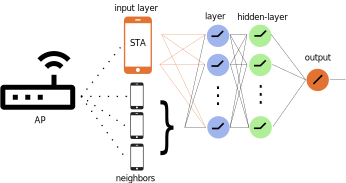
\includegraphics[width=\textwidth]{img/gossip-nn.pdf}
    \caption{Gossip STA throughput forecasting using
    neighboring STAs.}
    \label{fig:gossip}
\end{figure}
As shown in Figure~\ref{fig:gossip}, the input layer
contains features about the STA which throughput we
want to predict, as well as information of neighboring
STAs attached to the same AP.
The former features relate to data as the STA coordinates,
the used primary channel, or the experienced SINR;
whilst the latter relate to data related to neighboring
stations, such as the 1st quantile of the RSSI experienced
by the neighboring STAs.
See Tables~\ref{table:input} and \ref{table:output}
for further details.

Gossip allows to select which features should be used
in the forecasting process. In ITU-ML5G-PS-013 NETCOM
submission these were the selected features:
$X=(x_7,x_8,x_9,x_{10+2k},x_{15+2k},x_{20+2k},x_{21+2k})$.
The used NN was trained using the RMSprop gradient
descend method, Mean Squared Error (MSE) as
loss function, 50 training episodes, and a batch size
of 50 STAs.
Thanks to Gossip design, the training dataset is populated
with every STA of every deployment present among all
scenarios. Thus, the trained model submited to
ITU-ML5G-PS-013 used every STAs' $X$ features.
The training achieved a MSE of $\sim 23$.





\section{Insights}
In this section it is shown the behaviour of Gossip
in the ITU-ML5G-PS-013 training dataset.
Figure~\ref{fig:stas} and Figure~\ref{fig:aps} were
derived using a training dataset populated with the 80\% of each
scenario deployments, and a testing dataset populated with
the 20\% of each scenario deployments (both datasets
were derived using the ITU-ML5G-PS-013 training dataset
v4).
The figures correspond to the forecastings
performed in depployment080 of each scenario in the
created testing dataset.

\begin{figure}[h!]%
    \centering
    \subfloat[][]{%
        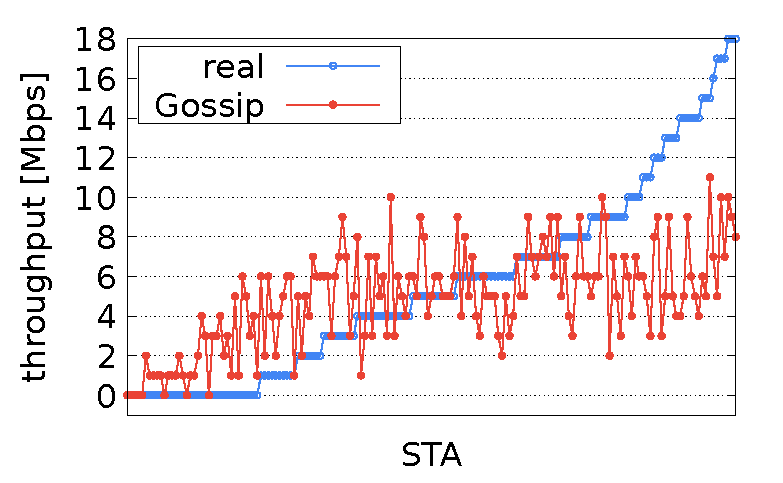
\includegraphics[width=0.3\textwidth]{img/sta-sce1a-dep080-results.eps}
        \label{fig:E2E-delay-evolution}%
    }% 1A
    \subfloat[][]{%
        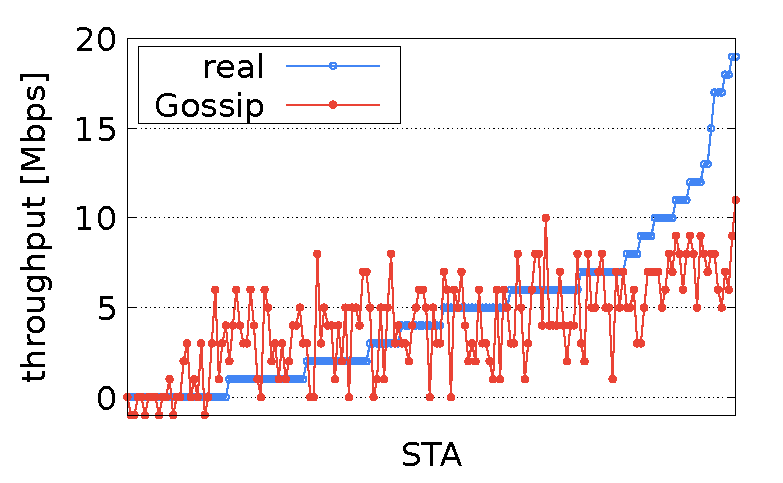
\includegraphics[width=0.3\textwidth]{img/sta-sce1b-dep080-results.eps}
        \label{fig:provisioning-comparison}%
    }% 1B
    \subfloat[][]{%
        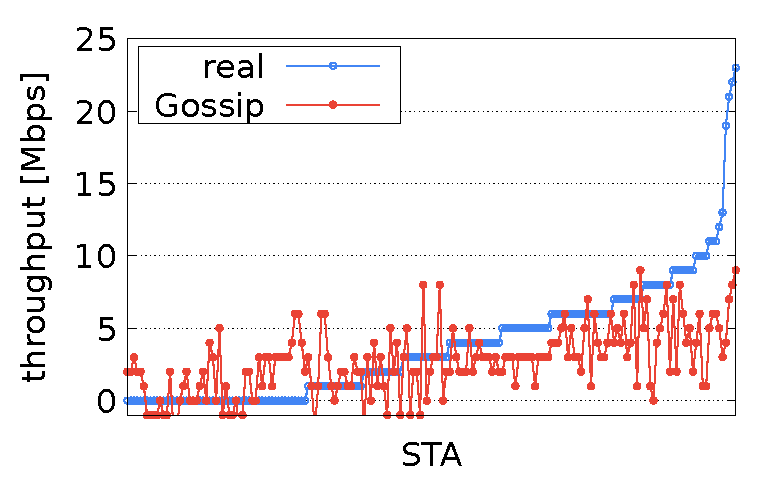
\includegraphics[width=0.3\textwidth]{img/sta-sce1c-dep080-results.eps}
        \label{fig:E2E-delay-evolution}%
    }\\ %1C
    \subfloat[][]{%
        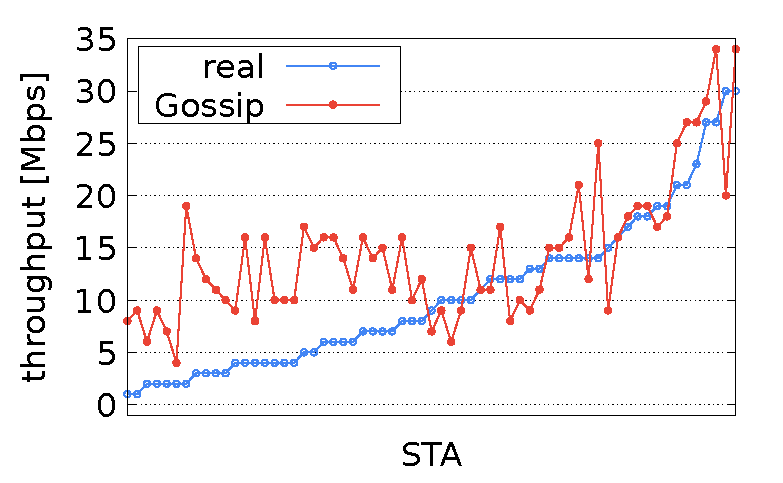
\includegraphics[width=0.3\textwidth]{img/sta-sce2a-dep080-results.eps}
        \label{fig:E2E-delay-evolution}%
    }% 2A
    \subfloat[][]{%
        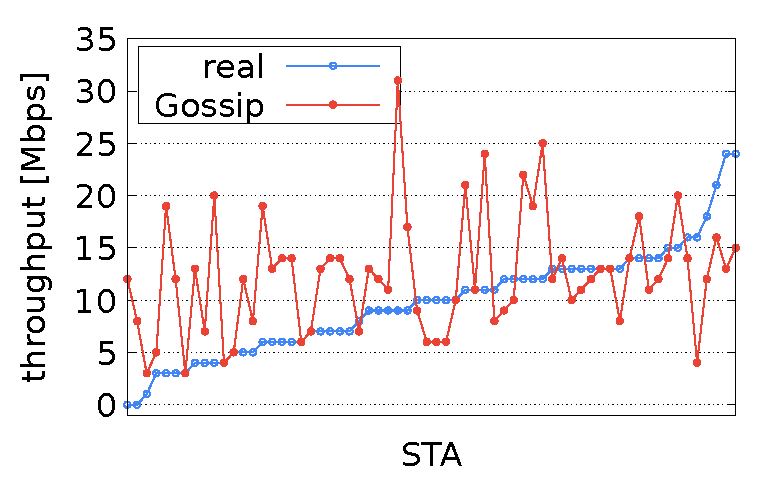
\includegraphics[width=0.3\textwidth]{img/sta-sce2b-dep080-results.eps}
        \label{fig:provisioning-comparison}%
    }% 2B
    \subfloat[][]{%
        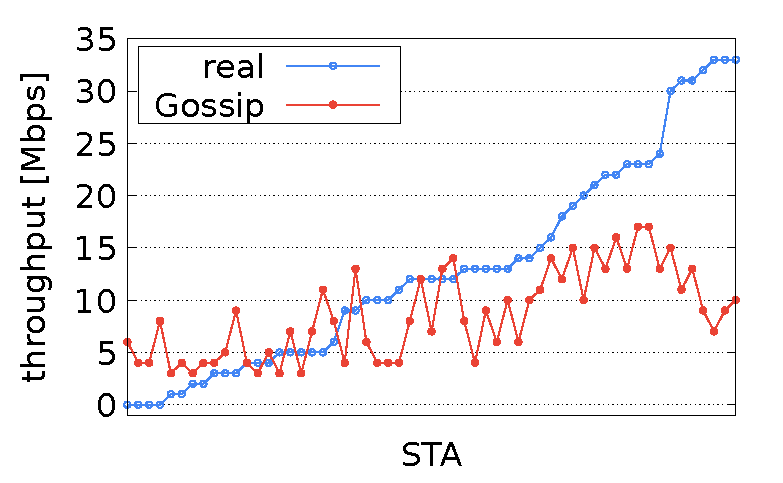
\includegraphics[width=0.3\textwidth]{img/sta-sce2c-dep080-results.eps}
        \label{fig:E2E-delay-evolution}%
    }\\ %2C
    \caption[]{Real (blue) and forecasted (red) througputs
    of each STA in deployment080 of (a) sce1a, (b) sce1b,
    (c) sce1c, (d) sce2a, (e) sce2c. STAs are arranged
    in the x-axis in increasing order or throughput.}
    \label{fig:stas}%
\end{figure}

Figure~\ref{fig:stas} shows the results of Gossip
forecasting on each different scenario, and it is clear
that Gossip remains near the average throughput reported
on each scenario as a consequence of using the MSE loss.
However, in scenario2a (Figure~\ref{fig:stas}(d)) the Gossip forecastings slightly decrease/increase
above the average throughput for the STAs will lowest/highest
throughput, respectively.






\begin{figure}[h!]%
    \centering
    \subfloat[][]{%
        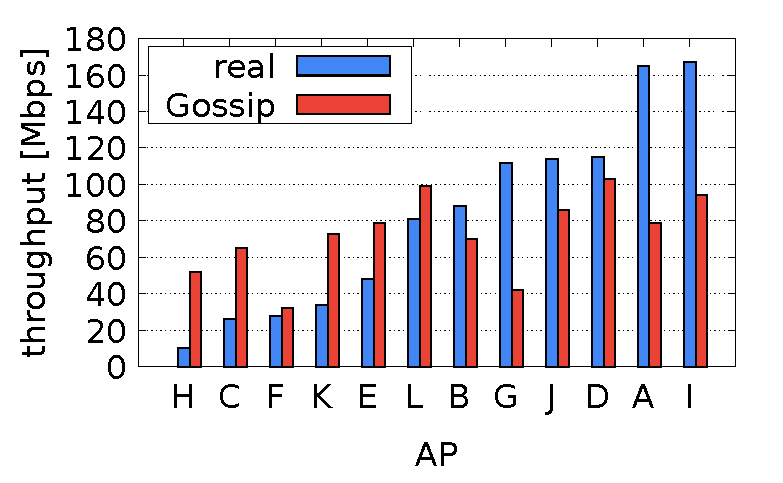
\includegraphics[width=0.3\textwidth]{img/aps-sce1a-dep080-results.eps}
        \label{fig:E2E-delay-evolution}%
    }% 1A
    \subfloat[][]{%
        \includegraphics[width=0.3\textwidth]{img/aps-sce1b-dep080-results.eps}
        \label{fig:provisioning-comparison}%
    }% 1B
    \subfloat[][]{%
        \includegraphics[width=0.3\textwidth]{img/aps-sce1c-dep080-results.eps}
        \label{fig:E2E-delay-evolution}%
    }\\ %1C
    \subfloat[][]{%
        \includegraphics[width=0.3\textwidth]{img/aps-sce2a-dep080-results.eps}
        \label{fig:E2E-delay-evolution}%
    }% 2A
    \subfloat[][]{%
        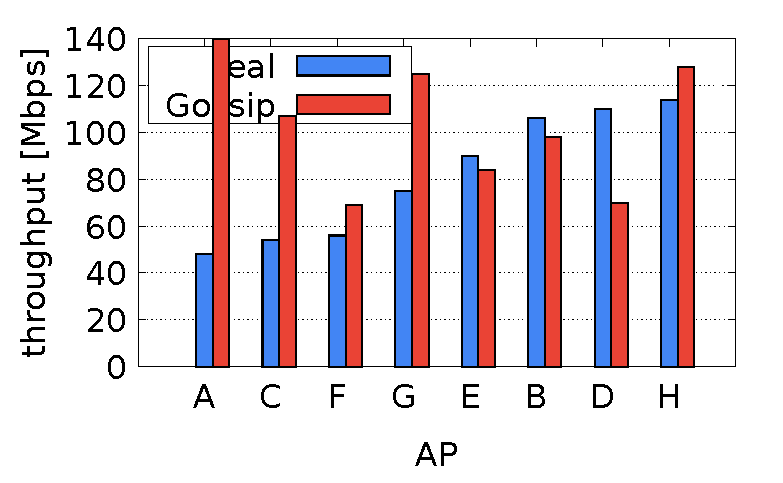
\includegraphics[width=0.3\textwidth]{img/aps-sce2b-dep080-results.eps}
        \label{fig:provisioning-comparison}%
    }% 2B
    \subfloat[][]{%
        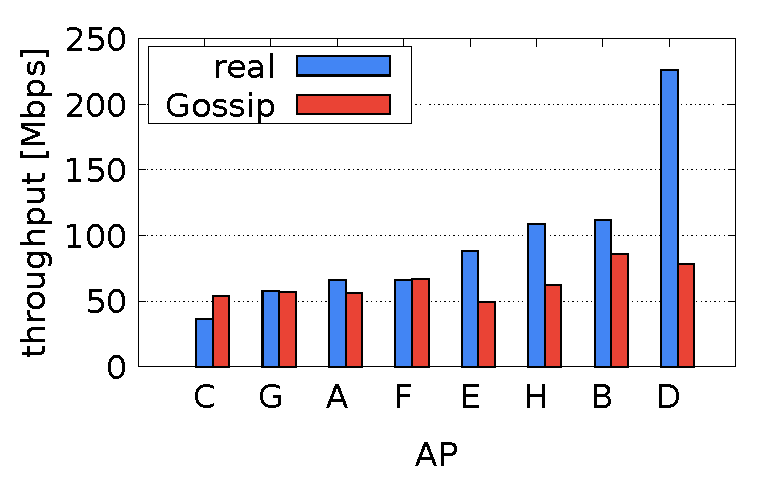
\includegraphics[width=0.3\textwidth]{img/aps-sce2c-dep080-results.eps}
        \label{fig:E2E-delay-evolution}%
    }\\ %2C
    \caption[]{Real (blue) and forecasted (red) througputs
    of each AP in deployment080 of (a) sce1a, (b) sce1b,
    (c) sce1c, (d) sce2a, (e) sce2c. APs are arranged
    in the x-axis in increasing order or throughput.}
    \label{fig:aps}%
\end{figure}

Nevertheless, ITU-ML5G-PS-013 asked to report the per-AP $\alpha$
throughput forecasting, i.e., which is derived as
a sum of the forecasted throughput for the attached
STAs $\hat{y}_\alpha = \sum_s \hat{y}_s$.
Figure~\ref{fig:aps} depicts the APs throughput
forecasts, and every scenario shows that Gossip still
keeps around the average throughput on each scenario,
and does not follow that much the increasing tendency
of the APs with higher throughputs.
Once again, results suggest that this behaviour might
be caused do to the usage of the MSE as loss function.

Furthermore, APs with higher throughput values are more
likely to have more channels being used, as they have
higher number of attached STAs.
But the solution submitted to ITU-ML5G-PS-013 only
used the features related to channels 0 and 1, i.e.,
features $x_9, x_{10}$, respectively.
Hence, Gossip missed the information of channels above
1, and that might have worsen the differentiation of
APs with many attached STAs, and higher number of
used channels.


\section{Conclusions}
Gossip is independent of the scenario size, and
its training can mix heterogeneous network conditions
so as to generalize the throughput forecasting.
However, the selected combination of features,
optimizer, NN, and metric resulted into forecasting
values near the mean throughput experienced in
the training set.

It is left as future work the search of NNs with
better performance, so as the hyper-parameters,
and training metric selected.
Immediate next steps would be to use other loss
functions to prevent Gossip being allways near the
average throughput in the scenario; and to feed it with
features related to every channel, and not only channel
0 and 1.
This way, Gossip might differentiate APs with lower/higher
number of attached STAs.\\
As latest remark, it might be a good idea to try out
regression methods accounting for features correlation
$\prod_ix_i$, or even use GRU neurons to ease the
differentiation of low/highly loaded APs by using a neuron gate.


\end{document}

